\documentclass[aspectratio=169]{beamer}
\usetheme{Madrid}
\usecolortheme{beaver}

% Packages
\usepackage{amsmath,amssymb,amsthm}
\usepackage{algorithm}
\usepackage{algpseudocode}
\usepackage{tikz}
\usepackage{pgfplots}
\usepackage{booktabs}
\usepackage{multirow}
\usepackage{graphicx}
\usepackage{xcolor}
\usepackage[utf8]{inputenc}
\DeclareUnicodeCharacter{2192}{\ensuremath{\rightarrow}}
\DeclareUnicodeCharacter{2194}{\ensuremath{\leftrightarrow}}
\DeclareUnicodeCharacter{2265}{\ensuremath{\geq}}
\usepackage{hyperref}
% Prevent translator/hyperref interaction warnings in PDF strings
\pdfstringdefDisableCommands{\def\translate#1{#1}}
\usepackage{pifont} % provides \ding for checkmarks and dingbats

% Beamer/amsthm provide theorem-like environments; avoid redefinition here.
\pgfplotsset{compat=1.18}
\usetikzlibrary{graphs,arrows.meta,positioning,shapes}

% Custom colors
\definecolor{darkred}{RGB}{139,0,0}
\definecolor{darkgreen}{RGB}{0,100,0}
\definecolor{darkblue}{RGB}{0,0,139}

% Title page information
\title[Feedback Vertex Set]{The Feedback Vertex Set Problem:\\Theory, Algorithms, and Applications}
\subtitle{CSE472 Project Presentation - Group 6}
\author{2005090 -- Tawkir Aziz Rahman \\ 2005067 -- Suman Hossain \\ 2005074 -- Dipanta Kumar Roy Nobo \\ 2005091 -- Waseem Mustak Zisan \\ 2005104 -- Hasin Arafat \\ 2005109 -- Noushin Tabassum Aoishy}
\institute{Bangladesh University of Engineering and Technology \\ Department of CSE}
\date{\today}

% Custom commands
\newcommand{\fvs}{\textsc{FVS}}
\newcommand{\np}{\textsc{NP}}
\newcommand{\opt}{\textsc{OPT}}

\begin{document}

% Title slide
\begin{frame}
	\titlepage
\end{frame}

% Table of contents
\begin{frame}{Outline}
	\tableofcontents
\end{frame}













% ============================================
% PART 1: PROBLEM DEFINITION & VISUAL INTUITION
% ============================================

\section{Problem Definition and Visual Intuition}

% --------------------------------------------
\begin{frame}{Overview}
	\begin{block}{Goal of This Section}
		\begin{itemize}
			\item Understand what the Feedback Vertex Set (FVS) problem is
			\item Build intuition using cycles and forests
			\item Visualize how removing vertices eliminates cycles
		\end{itemize}
	\end{block}
\end{frame}

% --------------------------------------------
\begin{frame}{What is a Cycle?}

	\begin{block}{Definition}
		A \textbf{cycle} is a path that starts and ends at the same vertex without repeating edges.
	\end{block}

	\vspace{0.3cm}

	\begin{itemize}
		\item Cycles represent loops in a graph
		\item They create dependencies or redundancies
	\end{itemize}

	\vspace{0.3cm}

	\begin{alertblock}{Key Idea}
		If a graph has no cycles, it is called a \textbf{forest}.
	\end{alertblock}

\end{frame}

% --------------------------------------------
\begin{frame}{What is a Forest?}

	\begin{block}{Definition}
		A \textbf{forest} is a graph with no cycles (i.e., a collection of trees).
	\end{block}

	\vspace{0.3cm}

	\begin{itemize}
		\item Trees are connected acyclic graphs
		\item Forest = one or multiple disconnected trees
	\end{itemize}

	\vspace{0.3cm}

	\begin{alertblock}{Observation}
		Our goal in FVS is to transform any graph into a forest.
	\end{alertblock}

\end{frame}

% --------------------------------------------
\begin{frame}{Feedback Vertex Set (FVS)}

	\begin{definition}
		Given a graph $G = (V, E)$, a \textbf{Feedback Vertex Set} is a subset $S \subseteq V$ such that removing $S$ makes the graph acyclic.
	\end{definition}

	\vspace{0.3cm}

	\begin{block}{Objective}
		Find the \textbf{smallest possible} such set $S$.
	\end{block}

	\vspace{0.3cm}

	\begin{itemize}
		\item Remove vertices $\rightarrow$ eliminate cycles
		\item Minimize number of removed vertices
	\end{itemize}

\end{frame}

% --------------------------------------------
\begin{frame}{Problem Formulation}

	\begin{block}{Decision Version}
		\begin{itemize}
			\item Input: Graph $G = (V,E)$, integer $k$
			\item Question: Does there exist $S \subseteq V$ with $|S| \leq k$ such that $G-S$ is acyclic?
		\end{itemize}
	\end{block}

	\vspace{0.4cm}

	\begin{block}{Optimization Version}
		Find a minimum-size Feedback Vertex Set.
	\end{block}

\end{frame}




% --------------------------------------------
\begin{frame}{Visual Example: Tree (No Cycles)}

	\begin{center}
		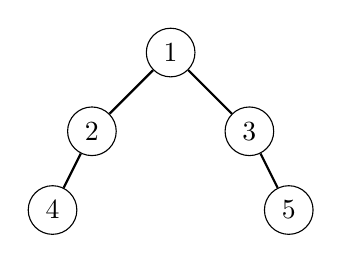
\begin{tikzpicture}[scale=1]
			\node[circle,draw] (1) at (0,1.5) {1};
			\node[circle,draw] (2) at (-1,0.5) {2};
			\node[circle,draw] (3) at (1,0.5) {3};
			\node[circle,draw] (4) at (-1.5,-0.5) {4};
			\node[circle,draw] (5) at (1.5,-0.5) {5};

			\draw[thick] (1) -- (2);
			\draw[thick] (1) -- (3);
			\draw[thick] (2) -- (4);
			\draw[thick] (3) -- (5);
		\end{tikzpicture}
	\end{center}

	\vspace{0.2cm}

	\begin{itemize}
		\item No cycles exist
		\item Graph is already a forest
	\end{itemize}

	\begin{alertblock}{Result}
		FVS = $\emptyset$
	\end{alertblock}

\end{frame}



% --------------------------------------------
\begin{frame}{Visual Example: Simple Cycle}

	\begin{center}
		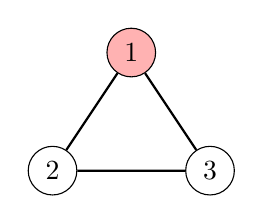
\begin{tikzpicture}[scale=1]
			\node[circle,draw,fill=red!30] (1) at (0,1.5) {1};
			\node[circle,draw] (2) at (-1,0) {2};
			\node[circle,draw] (3) at (1,0) {3};
			\draw[thick] (1) -- (2) -- (3) -- (1);
		\end{tikzpicture}
	\end{center}

	\vspace{0.2cm}

	\begin{itemize}
		\item This graph contains a cycle (triangle)
		\item Removing vertex 1 breaks the cycle
	\end{itemize}

	\begin{alertblock}{Result}
		FVS = $\{1\}$, size = 1
	\end{alertblock}

\end{frame}

% --------------------------------------------
\begin{frame}{Visual Example: Multiple Cycles}

	\begin{center}
		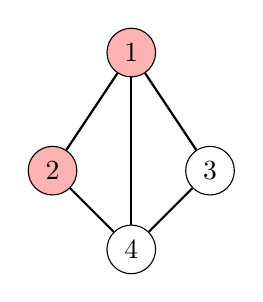
\begin{tikzpicture}[scale=1]
			\node[circle,draw,fill=red!30] (1) at (0,1.5) {1};
			\node[circle,draw,fill=red!30] (2) at (-1,0) {2};
			\node[circle,draw] (3) at (1,0) {3};
			\node[circle,draw] (4) at (0,-1) {4};

			\draw[thick] (1) -- (2) -- (4) -- (3) -- (1);
			\draw[thick] (1) -- (4);
		\end{tikzpicture}
	\end{center}

	\vspace{0.2cm}

	\begin{itemize}
		\item Multiple overlapping cycles exist
		\item Need to remove more vertices
	\end{itemize}

	\begin{alertblock}{Result}
		FVS = $\{1,2\}$
	\end{alertblock}

\end{frame}



% --------------------------------------------
% --------------------------------------------
\begin{frame}{Visual Example: Complex Graph $\rightarrow$ Forest}

	\begin{center}
		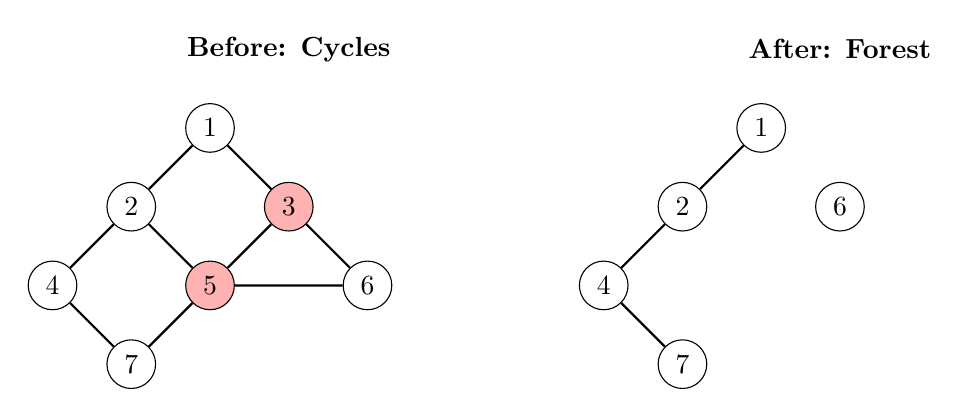
\begin{tikzpicture}[scale=1]
			% ---------------- Before (Left) ----------------
			\node at (-4,3) {\textbf{Before: Cycles}};

			% Nodes
			\node[circle,draw] (B1) at (-5,2) {1};
			\node[circle,draw] (B2) at (-6,1) {2};
			\node[circle,draw,fill=red!30] (B3) at (-4,1) {3};
			\node[circle,draw] (B4) at (-7,0) {4};
			\node[circle,draw,fill=red!30] (B5) at (-5,0) {5};
			\node[circle,draw] (B6) at (-3,0) {6};
			\node[circle,draw] (B7) at (-6,-1) {7};

			% Edges
			\draw[thick] (B1) -- (B2) -- (B4) -- (B7);
			\draw[thick] (B2) -- (B5) -- (B6);
			\draw[thick] (B3) -- (B5);
			\draw[thick] (B1) -- (B3) -- (B6);
			\draw[thick] (B5) -- (B7);

			% ---------------- After (Right) ----------------
			\node at (3,3) {\textbf{After: Forest}};

			% Nodes (removed 3 and 5)
			\node[circle,draw] (A1) at (2,2) {1};
			\node[circle,draw] (A2) at (1,1) {2};
			\node[circle,draw] (A4) at (0,0) {4};
			\node[circle,draw] (A6) at (3,1) {6};
			\node[circle,draw] (A7) at (1,-1) {7};

			% Edges (remaining)
			\draw[thick] (A1) -- (A2) -- (A4) -- (A7);
		\end{tikzpicture}
	\end{center}

	\vspace{0.2cm}

	\begin{itemize}
		\item \textbf{Before:} Multiple cycles exist, highlighted red vertices (3,5) are part of FVS.
		\item \textbf{After:} Removing FVS nodes breaks all cycles $\rightarrow$ Graph becomes a acyclic.
	\end{itemize}

	\begin{alertblock}{Final Verdict}
		FVS = $\{3,5\}$ $\rightarrow$ A set of vertices to remove all cycles.
	\end{alertblock}

\end{frame}






\begin{frame}{Visual Example: Complex Graph $\rightarrow$ Minimal FVS $\rightarrow$ Forest}

	\begin{columns}[T,onlytextwidth]
		% ----------------------------
		% Original Graph
		\column{0.48\textwidth}
		\begin{block}{Original Graph with Cycles}
			\begin{center}
				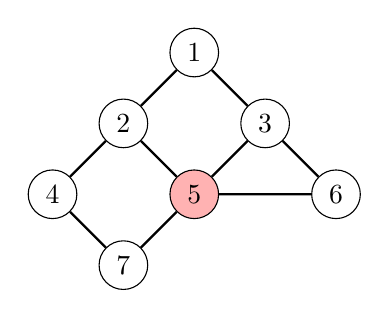
\begin{tikzpicture}[scale=0.9]
					% Nodes
					\node[circle,draw] (1) at (0,2) {1};
					\node[circle,draw] (2) at (-1,1) {2};
					\node[circle,draw] (3) at (1,1) {3};
					\node[circle,draw] (4) at (-2,0) {4};
					\node[circle,draw,fill=red!30] (5) at (0,0) {5};
					\node[circle,draw] (6) at (2,0) {6};
					\node[circle,draw] (7) at (-1,-1) {7};

					% Edges
					\draw[thick] (1) -- (2) -- (4) -- (7);
					\draw[thick] (2) -- (5) -- (6);
					\draw[thick] (3) -- (5);
					\draw[thick] (1) -- (3) -- (6);
					\draw[thick] (5) -- (7);
				\end{tikzpicture}
			\end{center}
		\end{block}

		% ----------------------------
		% Forest After Removing Minimal FVS
		\column{0.48\textwidth}
		\begin{block}{Resulting Forest (Remove 5)}
			\begin{center}
				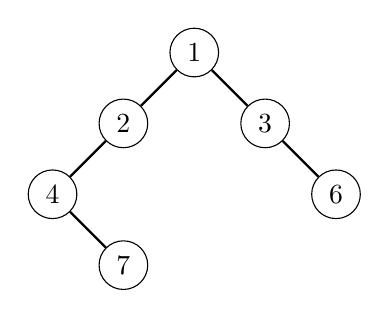
\begin{tikzpicture}[scale=0.9]
					% Nodes (excluding 5)
					\node[circle,draw] (1) at (0,2) {1};
					\node[circle,draw] (2) at (-1,1) {2};
					\node[circle,draw] (3) at (1,1) {3};
					\node[circle,draw] (4) at (-2,0) {4};
					\node[circle,draw] (6) at (2,0) {6};
					\node[circle,draw] (7) at (-1,-1) {7};

					% Edges (only remaining)
					\draw[thick] (1) -- (2) -- (4) -- (7);
					\draw[thick] (1) -- (3);
					\draw[thick] (3) -- (6);
				\end{tikzpicture}
			\end{center}
		\end{block}

	\end{columns}

	\vspace{0.2cm}

	\begin{itemize}
		\item Minimal Feedback Vertex Set: $\{5\}$
		\item Removing vertex 5 breaks all cycles $\rightarrow$ graph becomes a forest
	\end{itemize}

	\begin{alertblock}{Key Insight}
		Even if multiple vertices can break cycles, the \textbf{minimal FVS} is the set with the smallest size.
	\end{alertblock}

\end{frame}











% --------------------------------------------
\begin{frame}{Real-World Motivation}

	\begin{itemize}
		\item \textbf{Deadlocks in Operating Systems:} Cycles in resource allocation graph $\rightarrow$ remove critical process
		\item \textbf{Dependency Resolution:} Packages/modules with circular dependencies $\rightarrow$ remove one to break cycle
		\item \textbf{Circuit Design / Feedback Loops:} Loops in circuits $\rightarrow$ remove components to stabilize
		      % \item \textbf{Social Networks:} Removing influential nodes can break information loops
	\end{itemize}

	\vspace{0.3cm}

	\begin{alertblock}{Insight}
		FVS is a tool to identify minimal critical nodes whose removal resolves all cycles.
	\end{alertblock}

\end{frame}

% --------------------------------------------
\begin{frame}{Key Observations}

	\begin{itemize}
		\item Every cycle must contain at least one removed vertex
		\item Removing fewer vertices is always better
		\item Problem becomes harder as graph becomes denser
	\end{itemize}

	\vspace{0.4cm}

	\begin{block}{Core Insight}
		FVS is about selecting a minimum set of vertices that "hit" all cycles.
	\end{block}

\end{frame}

% % --------------------------------------------
% \begin{frame}{Summary of Intuition}

% \begin{itemize}
%   \item Cycles = structures we want to eliminate
%   \item Removing vertices breaks cycles
%   \item Goal: achieve an acyclic graph (forest)
%   \item Minimize number of removed vertices
% \end{itemize}

% \vspace{0.4cm}

% \begin{alertblock}{Takeaway}
% Feedback Vertex Set = Minimum set of vertices whose removal destroys all cycles.
% \end{alertblock}

% \end{frame}







% ============================================
% PART 2: COMPLEXITY & NP-COMPLETENESS
% ============================================

\section{Complexity and NP-Completeness}

% --------------------------------------------
\begin{frame}{Complexity Overview}

	\begin{block}{Goal of This Section}
		\begin{itemize}
			\item Analyze the \textbf{computational complexity} of FVS
			\item Understand decision vs optimization versions
			\item Prove NP-Completeness using reductions
		\end{itemize}
	\end{block}

\end{frame}

% --------------------------------------------
\begin{frame}{Decision vs Optimization}

	\begin{block}{Decision Version}
		Given $G, k$: Does there exist an FVS of size $\leq k$?
	\end{block}

	\begin{alertblock}{Fact}
		Decision version is \textbf{NP-Complete}
	\end{alertblock}

	\vspace{0.3cm}

	\begin{block}{Optimization Version}
		Find the minimum-size FVS
	\end{block}

	\begin{alertblock}{Fact}
		Optimization version is \textbf{NP-Hard}
	\end{alertblock}

\end{frame}

% --------------------------------------------
\begin{frame}{Main Claim}

	\begin{alertblock}{Theorem}
		The decision version of Feedback Vertex Set is \textbf{NP-Complete}.
	\end{alertblock}

	\vspace{0.3cm}

	\begin{block}{Proof Strategy}
		\begin{enumerate}
			\item Show FVS $\in$ NP
			\item Reduce Vertex Cover $\leq_p$ FVS
		\end{enumerate}
	\end{block}

\end{frame}

% --------------------------------------------
\begin{frame}{Step 1: FVS is in NP}

	\begin{block}{Key Idea (NP Definition)}
		A problem is in NP if a solution can be \textbf{verified in polynomial time}.
	\end{block}

	\vspace{0.3cm}

	\begin{itemize}
		\item Given a set $S$
		\item Remove $S$ from graph
		\item Check if graph has cycles (DFS)
	\end{itemize}

	\vspace{0.3cm}

	\begin{block}{Time Complexity}
		$O(V + E)$
	\end{block}

	\vspace{0.3cm}

	\begin{alertblock}{Conclusion}
		FVS $\in$ NP (verification is polynomial)
	\end{alertblock}

\end{frame}

% --------------------------------------------
\begin{frame}{Step 2: Reduction (VC $\rightarrow$ FVS)}

	\begin{block}{Known Fact}
		Vertex Cover is NP-Complete
	\end{block}

	\vspace{0.3cm}

	\begin{block}{Goal}
		Transform VC instance into FVS instance
	\end{block}

	\vspace{0.3cm}

	\begin{itemize}
		\item Each edge becomes a cycle
		\item FVS must break all cycles
	\end{itemize}

\end{frame}

% ----------------------------------
\begin{frame}{Step 2: Reduction (VC $\rightarrow$ FVS)}
	\begin{block}{Vertex Cover (VC) Problem}
		Find smallest $S \subseteq V$ such that every edge has at least one endpoint in $S$.
	\end{block}

	\vspace{0.3cm}

	\textbf{Construction:} Given VC instance $(G,k)$
	\begin{enumerate}
		\item For each edge $e = (u,v) \in E(G)$:
		      \begin{itemize}
			      \item Add new vertex $w_e$
			      \item Form triangle: edges $(u,v)$, $(u,w_e)$, $(v,w_e)$
		      \end{itemize}
		\item Keep same parameter $k' = k$
	\end{enumerate}

	\vspace{0.3cm}

	\begin{theorem}
		$G$ has VC of size $\leq k$ $\Leftrightarrow$ $G'$ has \fvs\ of size $\leq k$
	\end{theorem}

	\textbf{Time:} $O(|E|)$ (polynomial)
\end{frame}


% --------------------------------------------
\begin{frame}{Reduction Construction (Graph)}

	\begin{center}
		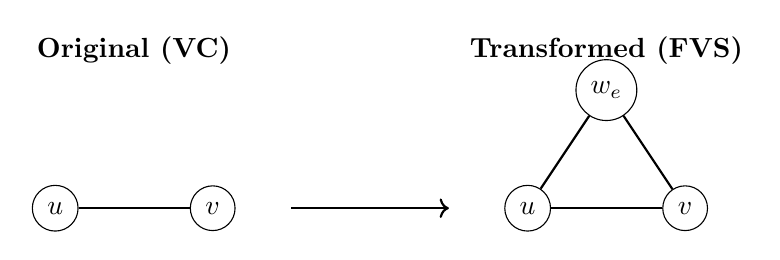
\begin{tikzpicture}[scale=1]

			\node at (-3,2) {\textbf{Original (VC)}};

			\node[circle,draw] (u) at (-4,0) {$u$};
			\node[circle,draw] (v) at (-2,0) {$v$};

			\draw[thick] (u) -- (v);

			\draw[->,thick] (-1,0) -- (1,0);

			\node at (3,2) {\textbf{Transformed (FVS)}};

			\node[circle,draw] (u2) at (2,0) {$u$};
			\node[circle,draw] (v2) at (4,0) {$v$};
			\node[circle,draw] (w) at (3,1.5) {$w_e$};

			\draw[thick] (u2) -- (v2);
			\draw[thick] (u2) -- (w);
			\draw[thick] (v2) -- (w);

		\end{tikzpicture}
	\end{center}

	\vspace{0.3cm}

	\begin{itemize}
		\item Each edge becomes a triangle
		\item Triangle = cycle $\rightarrow$ must be broken
	\end{itemize}

\end{frame}

% --------------------------------------------
% ✅ ADDED YOUR BIG VISUAL (KEEPING IT)
% --------------------------------------------
\begin{frame}{VC $\rightarrow$ FVS: Full Graph Illustration}

	\begin{columns}[T]
		\column{0.45\textwidth}

		\textbf{Original Graph}
		\begin{center}
			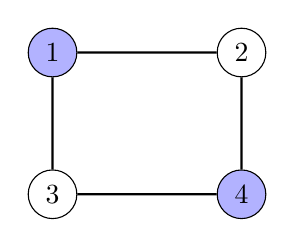
\begin{tikzpicture}[scale=1.2]
				\node[circle,draw,fill=blue!30] (1) at (0,1.5) {1};
				\node[circle,draw] (2) at (2,1.5) {2};
				\node[circle,draw] (3) at (0,0) {3};
				\node[circle,draw,fill=blue!30] (4) at (2,0) {4};

				\draw[thick] (1)--(2)--(4)--(3)--(1);
			\end{tikzpicture}
		\end{center}

		\small VC = $\{1,4\}$

		\column{0.55\textwidth}

		\textbf{Transformed Graph}
		\begin{center}
			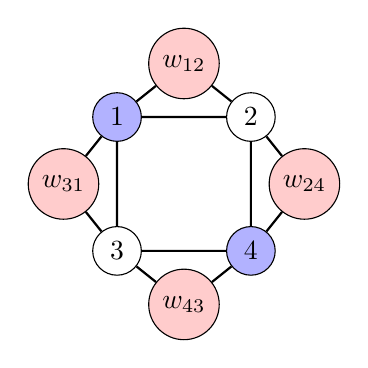
\begin{tikzpicture}[scale=0.85]
				\node[circle,draw,fill=blue!30] (1) at (0,2) {1};
				\node[circle,draw] (2) at (2,2) {2};
				\node[circle,draw] (3) at (0,0) {3};
				\node[circle,draw,fill=blue!30] (4) at (2,0) {4};

				\node[circle,draw,fill=red!20] (w12) at (1,2.8) {$w_{12}$};
				\node[circle,draw,fill=red!20] (w24) at (2.8,1) {$w_{24}$};
				\node[circle,draw,fill=red!20] (w43) at (1,-0.8) {$w_{43}$};
				\node[circle,draw,fill=red!20] (w31) at (-0.8,1) {$w_{31}$};

				\draw[thick] (1)--(2)--(w12)--(1);
				\draw[thick] (2)--(4)--(w24)--(2);
				\draw[thick] (4)--(3)--(w43)--(4);
				\draw[thick] (3)--(1)--(w31)--(3);
			\end{tikzpicture}
		\end{center}

		\small Each triangle = one edge

	\end{columns}

	\vspace{0.3cm}

	\begin{block}{Key Insight}
		Breaking all triangles = covering all edges
	\end{block}

\end{frame}

% --------------------------------------------
\begin{frame}{Correctness of Reduction}

	\begin{block}{Claim}
		$G$ has a VC of size $\leq k$
		$\Longleftrightarrow$
		$G'$ has an FVS of size $\leq k$
	\end{block}

	\textbf{Forward:}
	\begin{itemize}
		\item VC selects endpoints $\rightarrow$ every triangle broken
	\end{itemize}

	\textbf{Backward:}
	\begin{itemize}
		\item FVS must hit each triangle
		\item Implies every edge is covered
	\end{itemize}

\end{frame}

% --------------------------------------------
\begin{frame}{Polynomial Time Reduction}

	\begin{itemize}
		\item Add one vertex per edge
		\item Linear size increase
	\end{itemize}

	\begin{alertblock}{Conclusion}
		Reduction runs in polynomial time
	\end{alertblock}

\end{frame}




\begin{frame}{Reverse Reduction (FVS $\rightarrow$ VC)}
	\begin{block}{Reverse Direction}
		Shows Vertex Cover and \fvs\ are polynomially equivalent
	\end{block}

	\vspace{0.3cm}

	\textbf{Construction:} Given \fvs\ instance $(G,k)$
	\begin{enumerate}
		\item Replace each vertex $v \in V$ with triangle $\{v_1, v_2, v_3\}$
		\item For each edge $(u,v) \in E$, connect triangles with cross edges
		\item Set $k' = 2|V| + k$
	\end{enumerate}

	\vspace{0.3cm}

	\begin{theorem}
		$G$ has \fvs\ of size $\leq k$ $\Leftrightarrow$ $G'$ has VC of size $\leq 2|V| + k$
	\end{theorem}

	\textbf{Key Insight:}
	\begin{itemize}
		\item Each triangle needs $\geq 2$ vertices in VC
		\item Triangles with 3 vertices in VC, $\leftrightarrow$ vertices in \fvs
	\end{itemize}
\end{frame}



\begin{frame}{\fvs $\rightarrow$ VC: Visual Example}

	\begin{block}{Idea}
		Show structural similarity between problems
	\end{block}

	\vspace{0.3cm}

	\begin{columns}
		\column{0.4\textwidth}

		\textbf{Original Graph}
		\begin{center}
			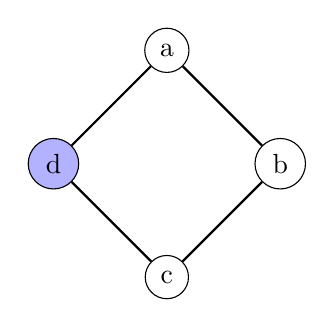
\begin{tikzpicture}[scale=1.2]
				\node[circle,draw] (a) at (90:1.2) {a};
				\node[circle,draw] (b) at (0:1.2) {b};
				\node[circle,draw] (c) at (270:1.2) {c};
				\node[circle,draw,fill=blue!30] (d) at (180:1.2) {d};

				\draw[thick] (a)--(b)--(c)--(d)--(a);
			\end{tikzpicture}
		\end{center}

		\small FVS = $\{d\}$

		\column{0.6\textwidth}

		\textbf{Construction}
		\begin{itemize}
			\item Each vertex $\rightarrow$ triangle
			\item Selecting all 3, $\leftrightarrow$ remove vertex
			\item Selecting 2, $\leftrightarrow$ keep vertex
		\end{itemize}

	\end{columns}

	\vspace{0.3cm}

	% \begin{alertblock}{Insight}
	% FVS and Vertex Cover are structurally related
	% \end{alertblock}

\end{frame}


\begin{frame}{\fvs $\rightarrow$ VC: Visual Example}
	\begin{columns}[T]
		\column{0.4\textwidth}
		\textbf{Original Graph $G$:}
		\begin{center}
			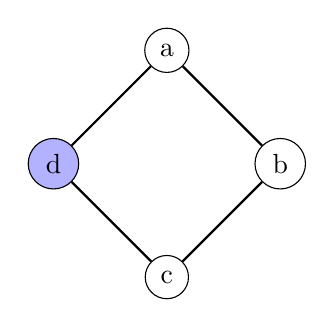
\begin{tikzpicture}[scale=1.2]
				\node[circle,draw] (a) at (90:1.2) {a};
				\node[circle,draw] (b) at (0:1.2) {b};
				\node[circle,draw] (c) at (270:1.2) {c};
				\node[circle,draw,fill=blue!30] (d) at (180:1.2) {d};
				\draw[thick] (a) -- (b) -- (c) -- (d) -- (a);
			\end{tikzpicture}
		\end{center}
		\small
		\fvs: $\{d\}$ (size=1)\\
		Removing $d$ breaks the 4-cycle

		\column{0.6\textwidth}
		\textbf{Transformed Graph $G'$:}
		\begin{center}
			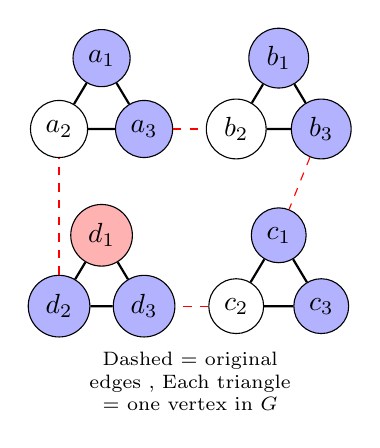
\begin{tikzpicture}[scale=0.9]
				% Triangles spaced out
				\node[circle,draw,fill=blue!30] (a1) at (0,2.5) {$a_1$};
				\node[circle,draw] (a2) at (-0.6,1.5) {$a_2$};
				\node[circle,draw,fill=blue!30] (a3) at (0.6,1.5) {$a_3$};
				\draw[thick] (a1) -- (a2) -- (a3) -- (a1);

				\node[circle,draw,fill=blue!30] (b1) at (2.5,2.5) {$b_1$};
				\node[circle,draw] (b2) at (1.9,1.5) {$b_2$};
				\node[circle,draw,fill=blue!30] (b3) at (3.1,1.5) {$b_3$};
				\draw[thick] (b1) -- (b2) -- (b3) -- (b1);

				\node[circle,draw,fill=red!30] (d1) at (0,0) {$d_1$};
				\node[circle,draw,fill=blue!30] (d2) at (-0.6,-1) {$d_2$};
				\node[circle,draw,fill=blue!30] (d3) at (0.6,-1) {$d_3$};
				\draw[thick] (d1) -- (d2) -- (d3) -- (d1);

				\node[circle,draw,fill=blue!30] (c1) at (2.5,0) {$c_1$};
				\node[circle,draw] (c2) at (1.9,-1) {$c_2$};
				\node[circle,draw,fill=blue!30] (c3) at (3.1,-1) {$c_3$};
				\draw[thick] (c1) -- (c2) -- (c3) -- (c1);

				% Representative cross edges (just show pattern)
				\draw[dashed,red] (a3) -- (b2);
				\draw[dashed,red] (b3) -- (c1);
				\draw[dashed,red] (c2) -- (d3);
				\draw[dashed,red] (d2) -- (a2);

				\node[text width=3cm,align=center,font=\scriptsize] at (1.25,-2) {\\Dashed = original edges , Each triangle = one vertex in $G$};
			\end{tikzpicture}
		\end{center}
	\end{columns}

	\vspace{0.3cm}
	\begin{minipage}{\textwidth}
		\small
		\textbf{Vertex Cover in $G'$:(with d1) is a FVS in  $G'$}
		% \begin{itemize}
		%   \item Choose \textbf{all 3} from triangle $d$ (blue) $\rightarrow$ vertex $d$ in \fvs
		%   \item Choose \textbf{2 from each} of triangles $a,b,c$ $\rightarrow$ vertices not in \fvs
		%   \item Total size = $3 + 2+2+2 = 9$
		%   \item Formula: $2|V| + k = 2\times4 + 1 = 9$ ✓
		% \end{itemize}
	\end{minipage}
\end{frame}
% --------------------------------------------
% ✅ YOUR SECOND VISUAL KEPT
% --------------------------------------------


% --------------------------------------------
\begin{frame}{Final Conclusion}

	\begin{block}{We Have Proven}
		\begin{itemize}
			\item FVS $\in$ NP
			\item Vertex Cover $\leq_p$ FVS
			\item VC is NP-Complete
		\end{itemize}
	\end{block}

	\vspace{0.4cm}

	\begin{alertblock}{Final Verdict}
		\textbf{Feedback Vertex Set (Decision) is NP-Complete}
	\end{alertblock}

	\vspace{0.3cm}

	\begin{block}{Implication}
		\begin{itemize}
			\item Optimization version is NP-Hard
			\item No known polynomial-time exact algorithm
		\end{itemize}
	\end{block}

\end{frame}


\begin{frame}{Algorithm Selection Criteria}
	\begin{columns}[T]
		\column{0.36\textwidth}
		\begin{block}{Essential Criteria}
			\footnotesize
			\textbf{1. Implementability}
			\begin{itemize}
				\item Feasible in 6-week timeframe
				\item Well-documented in literature
				\item Reasonable debugging complexity
			\end{itemize}

			\textbf{2. Research Potential}
			\begin{itemize}
				\item Novel comparisons possible
				\item Room for improvements
				\item Publishable results
			\end{itemize}

			\textbf{3. Complementary Nature}
			\begin{itemize}
				\item Different problem sizes
				\item Different paradigms
				\item Interesting comparisons
			\end{itemize}
		\end{block}

		\column{0.36\textwidth}
		\begin{block}{Additional Criteria}
			\footnotesize
			\textbf{4. Practical Relevance}
			\begin{itemize}
				\item Real-world applications
				\item Industry interest
				\item Addresses practical needs
			\end{itemize}

			\textbf{5. Educational Value}
			\begin{itemize}
				\item Learn important techniques
				\item Transferable skills
				\item Deep algorithmic insights
			\end{itemize}
		\end{block}

		\begin{alertblock}{Goal}
			\footnotesize
			Select algorithms that maximize research impact while ensuring feasibility
		\end{alertblock}
	\end{columns}
\end{frame}

\begin{frame}{Selected Algorithms for Implementation}
	\begin{block}{Three-Algorithm Approach (Maximum Research Impact)}
		We will implement three complementary algorithms covering the entire solution spectrum:
	\end{block}

	\vspace{0.3cm}

	\begin{enumerate}
		\item \textbf{Iterative Compression} (Exact FPT Algorithm)
		      \begin{itemize}
			      \footnotesize
			      \item Guarantees optimal solution for small-medium $k$
			      \item Time: $O(5^k \cdot kn^2)$ --- FPT breakthrough (2004)
			      \item Research: Hybrid approaches, parallelization, adaptive branching
		      \end{itemize}

		      \vspace{0.2cm}

		\item \textbf{Kernelization + Bounded Search Tree} (Enhanced Exact)
		      \begin{itemize}
			      \footnotesize
			      \item Preprocessing with reduction rules + exact search
			      \item Kernel reduction: 50-90\% for many graph types
			      \item Research: New reduction rules, smart branching strategies
		      \end{itemize}

		      \vspace{0.2cm}

		\item \textbf{Memetic Algorithm} (Advanced GA + Local Search)
		      \begin{itemize}
			      \footnotesize
			      \item Handles large instances (n $>$ 1000)
			      \item Combines population evolution with local optimization
			      \item Research: Problem-specific operators, ML integration, hybrid exact-metaheuristic
		      \end{itemize}
	\end{enumerate}
\end{frame}

\begin{frame}{Algorithm 1: Iterative Compression (IC)}
	\begin{columns}[T]
		\column{0.48\textwidth}
		\begin{block}{Core Concept}
			\footnotesize
			Given FVS of size $k+1$, compress it to size $k$ through smart enumeration
		\end{block}

		\textbf{Theoretical Significance:}
		\begin{itemize}
			\footnotesize
			\item Most important FPT technique
			\item Published in STOC/FOCS
			\item Demonstrates advanced understanding
		\end{itemize}

		\vspace{0.2cm}

		\textbf{Implementation:}
		\begin{itemize}
			\footnotesize
			\item Complexity: Medium
			\item Expected range: $k \leq 30$
			\item Validation on small instances
		\end{itemize}

		\column{0.48\textwidth}
		\textbf{Research Directions:}
		\begin{enumerate}
			\footnotesize
			\item \textbf{Hybrid Kernelization + IC}
			      \begin{itemize}
				      \scriptsize
				      \item Apply reduction rules before IC
				      \item Potential 2-5x speedup
			      \end{itemize}

			\item \textbf{Adaptive Branching}
			      \begin{itemize}
				      \scriptsize
				      \item Learn which vertices to branch first
				      \item Use graph structure metrics
			      \end{itemize}

			\item \textbf{Parallelization}
			      \begin{itemize}
				      \scriptsize
				      \item Independent branches in parallel
				      \item Multi-core speedup potential
			      \end{itemize}

			\item \textbf{Improved Compression}
			      \begin{itemize}
				      \scriptsize
				      \item Smart partition enumeration
				      \item Structure-based pruning
			      \end{itemize}
		\end{enumerate}

	\end{columns}
\end{frame}

\begin{frame}{Iterative Compression for FVS}
	\small
	\textbf{Idea:} Build solution incrementally and compress when too large.

	\textbf{Algorithm}
	{\small
		\setlength{\baselineskip}{8pt}
		\begin{algorithmic}[1]
			\State Order vertices $v_1,\dots,v_n$
			\State $F \gets \{v_1\}$
			\For{$i = 2$ to $n$}
			\State $F \gets F \cup \{v_i\}$
			\If{$|F| = k+1$}
			\ForAll{partitions $(F_1,F_2)$ of $F$}
			\State find $Y \subseteq V \setminus F_2$
			\If{$F_1 \cup Y$ is an FVS}
			\State update $F$ and \textbf{break}
			\EndIf
			\EndFor
			\If{no update performed}
			\State \textbf{return NO}
			\EndIf
			\EndIf
			\EndFor
			\State \textbf{return} $F$ \textbf{if} $|F| \le k$
		\end{algorithmic}
	}


	\textbf{Key Insight:} Compress size $k\!+\!1$ to $k$ \\
	\textbf{Time:} $O(5^k \cdot n^2)$
\end{frame}

\begin{frame}{Simulation}
	\textbf{Simulation of FVS (k=2) on 5 vertices}

	% ---------- STEP 1 ----------
	\textbf{Step 1: $F=\{A\}$}
	\begin{center}

		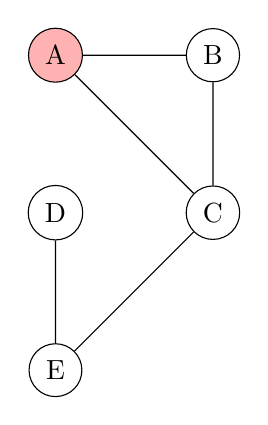
\begin{tikzpicture}[node distance=2cm]
			\node[draw, circle, fill=red!30] (A) {A};
			\node[draw, circle, right of=A] (B) {B};
			\node[draw, circle, below of=B] (C) {C};
			\node[draw, circle, left of=C] (D) {D};
			\node[draw, circle, below of=D] (E) {E};

			\draw (A)--(B)--(C)--(A);
			\draw (C)--(E)--(D);
		\end{tikzpicture}
	\end{center}

\end{frame}
\begin{frame}{Step 2: $F=\{A,B\}$}


	% ---------- STEP 2 ----------
	\begin{center}

		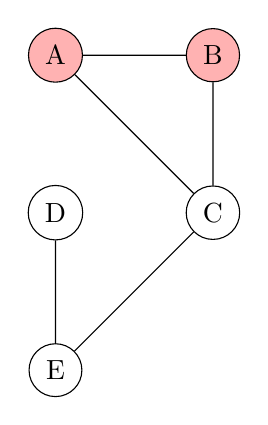
\begin{tikzpicture}[node distance=2cm]
			\node[draw, circle, fill=red!30] (A) {A};
			\node[draw, circle, fill=red!30, right of=A] (B) {B};
			\node[draw, circle, below of=B] (C) {C};
			\node[draw, circle, left of=C] (D) {D};
			\node[draw, circle, below of=D] (E) {E};

			\draw (A)--(B)--(C)--(A);
			\draw (C)--(E)--(D);
		\end{tikzpicture}
	\end{center}

\end{frame}
\begin{frame}{Step 3: $F=\{A,B,C\}$ (overflow)}

	% ---------- STEP 3 ----------
	\begin{center}

		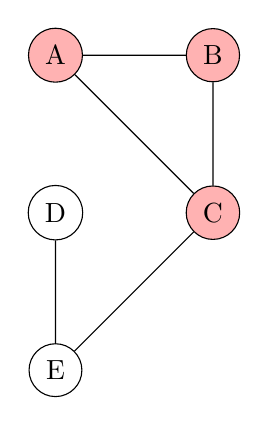
\begin{tikzpicture}[node distance=2cm]
			\node[draw, circle, fill=red!30] (A) {A};
			\node[draw, circle, fill=red!30, right of=A] (B) {B};
			\node[draw, circle, fill=red!30, below of=B] (C) {C};
			\node[draw, circle, left of=C] (D) {D};
			\node[draw, circle, below of=D] (E) {E};

			\draw (A)--(B)--(C)--(A);
			\draw (C)--(E)--(D);
		\end{tikzpicture}

	\end{center}
	\pause
	\textbf{Fix: Remove C $\Rightarrow F=\{A,B\}$}
\end{frame}

% -------- Slide 4 --------
\begin{frame}{Step 4: Add D (Overflow)}
	\begin{center}

		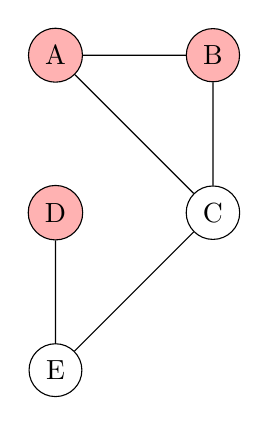
\begin{tikzpicture}[node distance=2cm]
			\node[draw, circle, fill=red!30] (A) {A};
			\node[draw, circle, fill=red!30, right of=A] (B) {B};
			\node[draw, circle, below of=B] (C) {C};
			\node[draw, circle, fill=red!30, left of=C] (D) {D};
			\node[draw, circle, below of=D] (E) {E};

			\draw (A)--(B)--(C)--(A);
			\draw (C)--(E)--(D);
		\end{tikzpicture}
	\end{center}


	\pause
	\textbf{Fix: Remove D $\Rightarrow F=\{A,B\}$}
\end{frame}

% -------- Slide 5 --------
\begin{frame}{Step 5: Add E (Overflow)}
	\begin{center}
		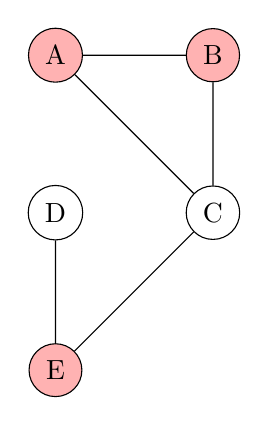
\begin{tikzpicture}[node distance=2cm]
			\node[draw, circle, fill=red!30] (A) {A};
			\node[draw, circle, fill=red!30, right of=A] (B) {B};
			\node[draw, circle, below of=B] (C) {C};
			\node[draw, circle, left of=C] (D) {D};
			\node[draw, circle, fill=red!30, below of=D] (E) {E};

			\draw (A)--(B)--(C)--(A);
			\draw (C)--(E)--(D);
		\end{tikzpicture}
	\end{center}

	\pause
	\textbf{Fix: Remove E $\Rightarrow F=\{A,B\}$}
\end{frame}

% -------- Final Slide --------
\begin{frame}{Final Answer}

	\begin{center}
		\begin{tikzpicture}[node distance=2cm]

			\node[draw, circle, below of=B] (C) {C};
			\node[draw, circle, left of=C] (D) {D};
			\node[draw, circle, below of=D] (E) {E};

			\draw (C)--(E)--(D);
		\end{tikzpicture}
	\end{center}

	\textbf{$F=\{A,B\}$}
\end{frame}






\begin{frame}{Algorithm 2: Kernelization + Bounded Search Tree}
	\begin{columns}[T]
		\column{0.48\textwidth}
		\begin{block}{Core Concept}
			\footnotesize
			Reduce graph size via preprocessing rules, then apply exact search on smaller kernel
		\end{block}

		\textbf{Reduction Rules:}
		\begin{itemize}
			\footnotesize
			\item Degree 0, 1, 2 vertices
			\item Self-loops, duplicate edges
			\item Crown decomposition
			\item Flower rule
		\end{itemize}

		\vspace{0.2cm}

		\textbf{Search Strategy:}
		\begin{itemize}
			\footnotesize
			\item Smart vertex selection
			\item Bounded depth: $k$
			\item Branching factor: $\leq 4$
		\end{itemize}

		\column{0.48\textwidth}
		\textbf{Research Directions:}
		\begin{enumerate}
			\footnotesize
			\item \textbf{New Reduction Rules}
			      \begin{itemize}
				      \scriptsize
				      \item Graph-specific rules
				      \item Theoretical contribution
			      \end{itemize}

			\item \textbf{Rule Application Order}
			      \begin{itemize}
				      \scriptsize
				      \item Optimize ordering
				      \item ML-based prediction
			      \end{itemize}

			\item \textbf{Kernelization Bounds}
			      \begin{itemize}
				      \scriptsize
				      \item Tighter bounds for special classes
				      \item Experimental validation
			      \end{itemize}

			\item \textbf{Smart Branching}
			      \begin{itemize}
				      \scriptsize
				      \item Centrality-based selection
				      \item ML-guided search
			      \end{itemize}
		\end{enumerate}

	\end{columns}
\end{frame}


\begin{frame}{Kernelization + Bounded Search Tree}
	\small
	\textbf{Idea:} Reduce the graph, then branch on remaining cycles.

	\textbf{Algorithm}
	{\small
		\setlength{\baselineskip}{8pt}
		\begin{algorithmic}[1]
			\State Apply reduction rules:
			\State \quad remove degree $\le 1$ vertices
			\State \quad contract degree-2 vertices
			\State \quad include self-loop vertices
			\State Obtain kernel $(G',k')$
			\State \textbf{function} Search$(G',k')$
			\If{$G'$ is acyclic}
			\State \textbf{return} solution
			\EndIf
			\If{$k' < 0$}
			\State \textbf{return NO}
			\EndIf
			\State find a cycle $C$
			\For{each $v \in C$}
			\State recurse on $(G' - v,\, k' - 1)$
			\EndFor
		\end{algorithmic}
	}
	\textbf{Key Insight:} Small kernel $\Rightarrow$ small search tree \\
	\textbf{Time:} $O(4^k + n^2)$
\end{frame}

%-------------------------------
% Frame 1: Original Graph
%-------------------------------
\begin{frame}{Step 1: Original Graph}
	\centering
	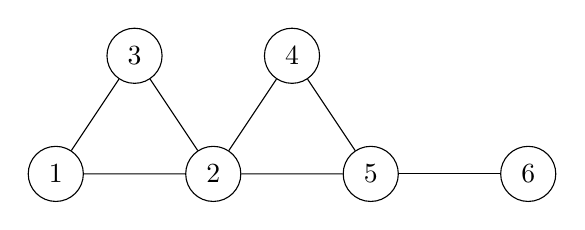
\begin{tikzpicture}[every node/.style={circle,draw,minimum size=7mm}]
		\node (1) at (0,0) {1};
		\node (2) at (2,0) {2};
		\node (3) at (1,1.5) {3};
		\node (4) at (3,1.5) {4};
		\node (5) at (4,0) {5};
		\node (6) at (6,0) {6};

		\draw (1)--(2)--(3)--(1);
		\draw (2)--(4)--(5)--(2);
		\draw (5)--(6);
	\end{tikzpicture}
\end{frame}

%-------------------------------
% Frame 2: Check degree <=1
%-------------------------------
\begin{frame}{Step 2: Remove degree $\leq$ 1 vertices}
	\centering
	\textbf{Vertex 6 removed}

	\vspace{0.5cm}

	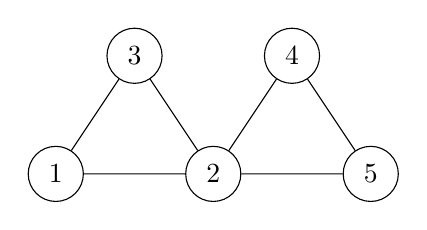
\begin{tikzpicture}[every node/.style={circle,draw,minimum size=7mm}]
		\node (1) at (0,0) {1};
		\node (2) at (2,0) {2};
		\node (3) at (1,1.5) {3};
		\node (4) at (3,1.5) {4};
		\node (5) at (4,0) {5};

		\draw (1)--(2)--(3)--(1);
		\draw (2)--(4)--(5)--(2);
	\end{tikzpicture}
\end{frame}

%-------------------------------
% Frame 3: Contract vertex 4
%-------------------------------
\begin{frame}{Step 3: Contract degree-2 vertex (4)}
	\centering
	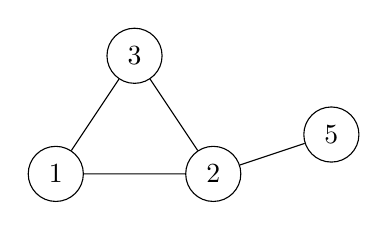
\begin{tikzpicture}[every node/.style={circle,draw,minimum size=7mm}]
		\node (1) at (0,0) {1};
		\node (2) at (2,0) {2};
		\node (3) at (1,1.5) {3};
		\node (5) at (3.5,0.5) {5};

		\draw (1)--(2)--(3)--(1);
		\draw (2)--(5);
	\end{tikzpicture}
\end{frame}

%-------------------------------
% Frame 4: Contract vertex 5
%-------------------------------
\begin{frame}{Step 4: Remove degree $\leq$ 1 vertex (5)}
	\centering
	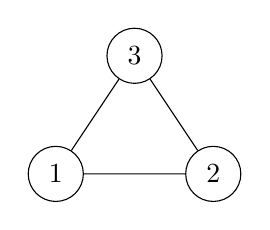
\begin{tikzpicture}[every node/.style={circle,draw,minimum size=7mm}]
		\node (1) at (0,0) {1};
		\node (2) at (2,0) {2};
		\node (3) at (1,1.5) {3};

		\draw (1)--(2)--(3)--(1);
	\end{tikzpicture}
\end{frame}

%-------------------------------
% Frame 5: Kernel obtained
%-------------------------------
\begin{frame}{Step 5: Kernel Graph (G')}
	\centering
	\textbf{Remaining cycle}

	\vspace{0.5cm}

	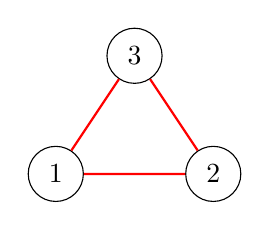
\begin{tikzpicture}[every node/.style={circle,draw,minimum size=7mm}]
		\node (1) at (0,0) {1};
		\node (2) at (2,0) {2};
		\node (3) at (1,1.5) {3};

		\draw[red, thick] (1)--(2)--(3)--(1);
	\end{tikzpicture}
\end{frame}

%-------------------------------
% Frame 6: Branch remove 1
%-------------------------------
\begin{frame}{Step 6: Branch - Remove vertex 1}
	\centering
	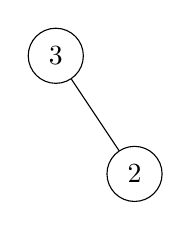
\begin{tikzpicture}[every node/.style={circle,draw,minimum size=7mm}]
		\node (2) at (2,0) {2};
		\node (3) at (1,1.5) {3};

		\draw (2)--(3);
	\end{tikzpicture}

	\vspace{0.5cm}
	Graph becomes acyclic
\end{frame}

%-------------------------------
% Frame 7: Branch remove 2
%-------------------------------
\begin{frame}{Step 7: Branch - Remove vertex 2}
	\centering
	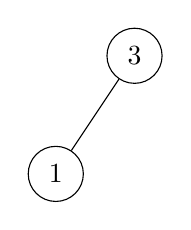
\begin{tikzpicture}[every node/.style={circle,draw,minimum size=7mm}]
		\node (1) at (0,0) {1};
		\node (3) at (1,1.5) {3};

		\draw (1)--(3);
	\end{tikzpicture}

	\vspace{0.5cm}
	Graph becomes acyclic
\end{frame}

%-------------------------------
% Frame 8: Branch remove 3
%-------------------------------
\begin{frame}{Step 8: Branch - Remove vertex 3}
	\centering
	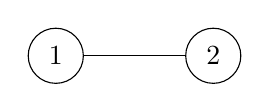
\begin{tikzpicture}[every node/.style={circle,draw,minimum size=7mm}]
		\node (1) at (0,0) {1};
		\node (2) at (2,0) {2};

		\draw (1)--(2);
	\end{tikzpicture}

	\vspace{0.5cm}
	Graph becomes acyclic
\end{frame}


\begin{frame}{Algorithm 3: Memetic Algorithm (GA + Local Search)}
	\begin{columns}[T]
		\column{0.48\textwidth}
		\begin{block}{Core Concept}
			\footnotesize
			Population evolution + local optimization for large-scale instances
		\end{block}

		\textbf{Components:}
		\begin{itemize}
			\footnotesize
			\item Smart initialization (greedy + random)
			\item FVS-aware crossover operators
			\item Centrality-based mutation
			\item Problem-specific local search
		\end{itemize}

		\vspace{0.2cm}

		\textbf{Practical Relevance:}
		\begin{itemize}
			\footnotesize
			\item Industry standard
			\item Handles $n > 1000$ vertices
			\item Near-optimal (5-10\% gap)
		\end{itemize}

		\column{0.48\textwidth}
		\textbf{Research Directions:}
		\begin{enumerate}
			\footnotesize
			\item \textbf{Cycle-Preserving Crossover}
			      \begin{itemize}
				      \scriptsize
				      \item Preserve cycle-breaking structures
				      \item Novel contribution
			      \end{itemize}

			\item \textbf{Hybrid Exact-Metaheuristic}
			      \begin{itemize}
				      \scriptsize
				      \item Use IC for small components
				      \item GA for large core
			      \end{itemize}

			\item \textbf{ML Integration}
			      \begin{itemize}
				      \scriptsize
				      \item Predict promising vertices
				      \item Learn operator selection
			      \end{itemize}

			\item \textbf{Multi-Objective}
			      \begin{itemize}
				      \scriptsize
				      \item Minimize size + maximize robustness
				      \item Pareto frontier
			      \end{itemize}
		\end{enumerate}

	\end{columns}
\end{frame}


\begin{frame}{Memetic Algorithm for FVS}
	\small
	\textbf{Idea:} Evolutionary search combined with local optimization.

	\textbf{Algorithm}
	\begin{algorithmic}[1]
		\State Encode solution as a permutation of vertices
		\State Decode by removing vertices until graph is acyclic
		\State Initialize population (greedy + random)
		\For{each generation}
		\State Evaluate fitness: $-|FVS|$
		\State Select parents (tournament)
		\State Crossover (cycle-aware)
		\State Mutation (swap cycle-heavy vertices)
		\State Local search (hill-climbing)
		\EndFor
		\State \textbf{return} best solution found
	\end{algorithmic}

	\textbf{Key Insight:} Exploration + refinement \\
	\textbf{Type:} Heuristic (near-optimal)
\end{frame}






%-------------------------------
% Frame 1: Original Graph
%-------------------------------
\begin{frame}{Step 1: Original Graph}
	\centering
	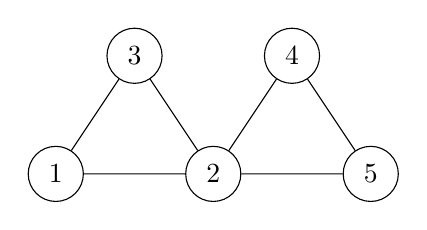
\begin{tikzpicture}[every node/.style={circle,draw,minimum size=7mm}]
		\node (1) at (0,0) {1};
		\node (2) at (2,0) {2};
		\node (3) at (1,1.5) {3};
		\node (4) at (3,1.5) {4};
		\node (5) at (4,0) {5};

		\draw (1)--(2)--(3)--(1);
		\draw (2)--(4)--(5)--(2);
	\end{tikzpicture}
\end{frame}

%-------------------------------
% Frame 2: Encoding (Permutation)
%-------------------------------
\begin{frame}{Step 2: Encode Solution}
	\centering
	Example permutation:

	\vspace{0.5cm}
	\Huge
	[3, 1, 5, 2, 4]
\end{frame}

%-------------------------------
% Frame 3: Decoding (Remove 3)
%-------------------------------
\begin{frame}{Step 3: Remove vertex 3}
	\centering
	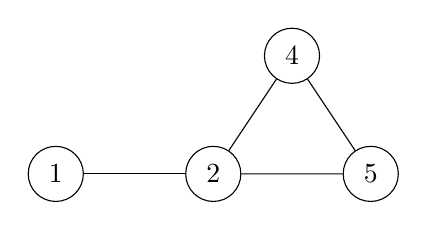
\begin{tikzpicture}[every node/.style={circle,draw,minimum size=7mm}]
		\node (1) at (0,0) {1};
		\node (2) at (2,0) {2};
		\node (4) at (3,1.5) {4};
		\node (5) at (4,0) {5};

		\draw (1)--(2);
		\draw (2)--(4)--(5)--(2);
	\end{tikzpicture}
\end{frame}

%-------------------------------
% Frame 4: Remove 1
%-------------------------------
\begin{frame}{Step 4: Remove vertex 1}
	\centering
	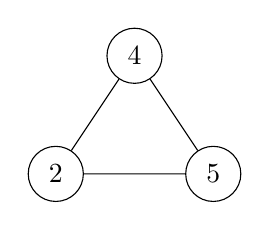
\begin{tikzpicture}[every node/.style={circle,draw,minimum size=7mm}]
		\node (2) at (2,0) {2};
		\node (4) at (3,1.5) {4};
		\node (5) at (4,0) {5};

		\draw (2)--(4)--(5)--(2);
	\end{tikzpicture}
\end{frame}


%-------------------------------
% Frame 5: Remove 5 (graph becomes acyclic)
%-------------------------------
\begin{frame}{Step 5: Remove vertex 5}
	\centering
	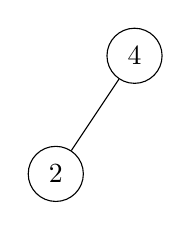
\begin{tikzpicture}[every node/.style={circle,draw,minimum size=7mm}]
		\node (2) at (2,0) {2};
		\node (4) at (3,1.5) {4};

		\draw (2)--(4);
	\end{tikzpicture}

	\vspace{0.5cm}
	Graph is now acyclic $\rightarrow$ Stop decoding
\end{frame}

%-------------------------------
% Frame 6: Fitness Evaluation
%-------------------------------
\begin{frame}{Step 6: Fitness Evaluation}
	\centering
	Removed vertices = \{3,1,5\}

	\vspace{0.5cm}
	Fitness = $-|FVS| = -3$
\end{frame}

%-------------------------------
% Frame 7: Selection
%-------------------------------
\begin{frame}{Step 7: Selection (Tournament)}
	\centering
	Select best solutions from population

	\vspace{0.5cm}
	Example:
	\[
		[3,1,5,2,4],\quad [2,4,1,5,3]
	\]
\end{frame}

%-------------------------------
% Frame 8: Crossover
%-------------------------------
\begin{frame}{Step 8: Crossover}
	\centering
	Parent 1: [3,1,5,2,4]

	Parent 2: [2,4,1,5,3]

	\vspace{0.5cm}
	Child:

	\Huge
	[3,4,1,2,5]
\end{frame}

%-------------------------------
% Frame 9: Mutation
%-------------------------------
\begin{frame}{Step 9: Mutation}
	\centering
	Before:

	\[
		[3,4,1,2,5]
	\]

	\vspace{0.5cm}
	After swap:

	\Huge
	[3,1,4,2,5]
\end{frame}

%-------------------------------
% Frame 10: Local Search
%-------------------------------
\begin{frame}{Step 10: Local Search}
	\centering
	Try improving solution:

	\vspace{0.5cm}
	Remove fewer vertices if possible

	\vspace{0.5cm}
	Example improvement:

	\Huge
	FVS size: 3 $\rightarrow$ 2
\end{frame}

%-------------------------------
% Frame 11: Final Solution
%-------------------------------
\begin{frame}{Step 11: Best Solution}
	\centering
	Best FVS found:

	\vspace{0.5cm}
	\Huge
	\{3,2\}

	\vspace{0.5cm}
	Graph becomes acyclic
\end{frame}






\end{document}

